\begin{enumerate}[label=\thesubsection.\arabic*.,ref=\thesubsection.\theenumi]
\numberwithin{equation}{enumi}

\item
Consider the unity feedback control system in Fig.  \ref{fig:ee18btech11038}. Find the value of K such that $PM = 30\degree$.

\begin{figure}[!ht]
	\begin{center}
		
		\resizebox{\columnwidth}{!}{The feedback current amplifier in Fig \ref{fig:ee18btech11038_probfig} utilizes two identical NMOS transistor sized so that at $I_{D1} = 0.2mA$, they operate at $V_{OV} = 0.2V$. Both the devices have $V_{t} =0.5V$ and $V_{A} = 10V$.
\begin{figure}[!ht]
	\begin{center}
		
		\resizebox{\columnwidth}{!}{\begin{circuitikz}[american]
\ctikzset{tripoles/mos style/arrows}
\draw  (0,0) node[ground](GND){} -- (0,1) to[isource, l= $I_{s}$] (0,3) -- (3,3) to[R=$R_{2}(14k\ohm$)] (4,3) -- (6,3)node{} to[R=$R_{1}(3.5k\ohm)$] (6,0) node[ground](GND){} (6,0);

\draw (3,6) node[nmos,](Q1){};
\draw (2,3) node[label={below:A}]{} to[short] (Q1.G);
\draw (Q1.center) node[right]{{$Q_{1}$}};
\draw (Q1.S) -- (3,5) node[ground](GND){};
\draw (3,9) node[vcc](VCC){} to [isource, l =$I(0.2mA)$ ](Q1.D);


\draw (6,7)node[nmos,](Q2){};
\draw (Q2.S) -- (6,3);
\draw (Q2.G) -- (3,7);
\draw (Q2.center) node[right]{{$Q_{2}$}};
\draw (6,9) node[vcc](VCC){} -- (Q2.D);
\draw (1,1)node[label = {below:$R_{in}$}]{} --(1,2);
\draw (1,2) to node[flowarrow]{}(2,2);

\draw (6.5,9.5) ++(0,0.001) node[flowarrow, rotate=-90]{\rotatebox{90}{$I_0$}};
\draw (7,8.7)node[label = {right:$R_{out}$}]{} --(6.5,8.7);
\draw (6.5,8.5) ++(0,-0.1) node[flowarrow, rotate=-90]{};
\end{circuitikz}}
	\end{center}
\caption{Problem Figure}
\label{fig:ee18btech11038_probfig}
\end{figure}
\begin{table}[!ht]
\centering
\input{./tables/ee18btech11038_given.tex}
\caption{Given Parameters}
\label{table: given}
\end{table}

\begin{enumerate}[label=(\alph*)]

\item  If $I_{S}$ has zero DC component, show that both $Q_{1}$ and $Q_{2}$ are, operating at $I_{D} = 0.2mA$. What is DC voltage at the input?
\\
\item Find $g_{m}$ and $r_{o}$ for each $Q_{1}$ and $Q_{2}$.
\\
\item  Find the open loop circuit and the value of $R_{i}$, $G$ and $R_{o}$.
\\
\item  Find the value of $H$.
\\
\item  Find $GH$ and $T$
\\
\item Find $R_{in}$ and $R_{out}$.
\end{enumerate}
%\renewcommand{\thefigure}{\theenumi.\arabic{figure}}


\begin{enumerate}[label=\arabic*.,ref=\theenumi]
\numberwithin{equation}{enumi}
\renewcommand{\thefigure}{\theenumi.\arabic{figure}}
\item Find the DC voltage at the node $A$.
\\
\solution 
Given that $I_{s}$ has zero DC component, it can be neglected in DC analysis of the circuit. The current does not enter the Gate terminal of any mosfet. Thus the DC current flow is as shown in Fig \ref{fig:ee18btech11038_dcckt} 
%Given $V_{OV} = 0.2V$ and  $V_{t} = 0.5V$, for Q1-
\begin{align}
    V_{GS1} = V_{OV}  + V_{t} = 0.7V\\
    \implies V_A = V_{G1} = V_{GS1} = 0.7V
    \end{align}
%a)DC analysis of circuit.\\
\begin{figure}[!ht]
	\begin{center}
		
		\resizebox{\columnwidth}{!}{\begin{circuitikz}[american]
\ctikzset{tripoles/mos style/arrows}
\draw (2,3) to[R=$R_{2}(14k\ohm$), i=$I_{dc}(0)$] (6,3) -- (6,3)node{} to[R=$R_{1}(3.5k\ohm)$] (6,0) node[ground](GND){} (6,0);

\draw (3,6) node[nmos,](Q1){};
\draw (2,3) node[]{} to[short] (Q1.G);
\draw (Q1.center) node[right]{{$Q_{1}$}};
\draw (Q1.S) to[short, i=$I_{D1}$](3, 5) -- (3,5) node[ground](GND){};
\draw (3,9) node[vcc](VCC){} to[short, i=$I_{D1}$](3,8.5) to[isource, l =$I(0.2mA)$ ](Q1.D);


\draw (6,7)node[nmos,](Q2){};
\draw (Q2.S) to[short, i=$I_{D2}$](6, 3) -- (6,3);
\draw (Q2.G) -- (3,7);
\draw (Q2.center) node[right]{{$Q_{2}$}};
\draw (6,9) node[vcc](VCC){} to[short, i=$I_{D2}$](6,8.5) -- (Q2.D);
\draw (2,3) to[short, -o] (2,2.5)node[below]{$V_{G1}$};
\draw (5,7) to[short, -o] (5,6.5)node[below]{$V_{G2}$};
\draw (6,3) to[short, -o] (6.5,3)node[right]{$V_{S2}$};
\draw (3,7) to[short, -o] (2.5,7)node[left]{$V_{D2}$};
\end{circuitikz}}
	\end{center}
\caption{DC Analysis Circuit}
\label{fig:ee18btech11038_dcckt}
\end{figure}
%
\item Show that the drain current for $Q2$ is $I_{D_2} = 0.2$mA.
\\
\solution 
\begin{align}
\because I_s &= 0 \text{ and }
\\
I_{G1} &= 0,
\end{align}
no current passes through $R_2$ and
%
\begin{align}
\because I_s &= 0 \text{ and }
\\
V_{S2} &=V_{A} = 0.7
\\
\implies I_{D2} &= \frac{V_{S2}}{R{1}} 
\\
I_{D2} &= 0.2mA
\end{align}

\item Find $g_{m}$ and $r_{o}$.\\
\solution 
\begin{align}
g_{m} &= \frac{2I_{D}}{V_{OV}} 
\\
 &=2 \, mA/V
\end{align}
and 
\begin{align}
    r_{0} &= \frac{V_{A}}{I_{D}}
\\
 &= 50k\ohm
\end{align}
%
\item Find $H$.
\\
\solution With port1 shorted in Fig. \ref{fig:ee18btech11038_smlckt},
\begin{figure}[!ht]
	\begin{center}
		
		\resizebox{\columnwidth}{!}{\begin{circuitikz}[american]
\ctikzset{tripoles/mos style/arrows}
\draw  (0,0) node[ground](GND){} -- (0,1) to[isource, l= $I_{s}$] (0,3) -- (3,3) to[R=$R_{2}(14k\ohm$), i=$I_{s}$] (6,3) -- (6,3)node{} to[R=$R_{1}(3.5k\ohm)$] (6,0) node[ground](GND){} (6,0);

\draw (3,6) node[nmos,](Q1){};
\draw (2,3)  to[short, i=$i(0)$] (Q1.G);
\draw (Q1.center) node[right]{{$Q_{1}$}};
\draw (Q1.S) -- (3,5) node[ground](GND){};
\draw (Q1.D) -- (3,7);
\draw (3,6.75) -- (4,6.75) to[R= $r_{o1}$](4,5.25) -- (3,5.25);



\draw (6,7)node[nmos,](Q2){};
\draw (Q2.S) to[short, i=$I_{o}$](6, 3) -- (6,3);
\draw (Q2.G) -- (3,7);
\draw (Q2.center) node[right]{{$Q_{2}$}};
\draw (6,9) node[ground, rotate=180]{} to[short, i=$I_{o}$](6,8.5) -- (Q2.D);
\draw (6,7.75) -- (7,7.75) to[R= $r_{o2}$](7,6.25) -- (6,6.25);

\draw (2,1)node[label = {below:$Port 1$}]{} --(2,2);
\draw (2,2) to node[flowarrow]{}(3,2);
\draw (2,3) to[short, -o] (2,2.5)node[below]{$v_{g1}$};
\draw (5,7) to[short, -o] (5,6.5)node[below]{$v_{g2}$};
\draw (6,3) to[short, -o] (6.5,3)node[right]{$v_{s2}$};
\draw (3,7) to[short, -o] (2.5,7)node[left]{$v_{d1}$};
\draw (7,5) ++(0,-0.1) node[flowarrow, rotate=-90]{\rotatebox{90}{$Port 2$}};
\draw[dashed] (3,1) to[short](3,4) to[short](8, 4) to[short](8,1) to[short](3,1);

\end{circuitikz}}
	\end{center}
\caption{Small Circuit Model}
\label{fig:ee18btech11038_smlckt}
\end{figure}

\begin{align}
    H &= \frac{I_{f}}{I_{0}}, 
\\
     &= \frac{R_{1}}{R_{1} + R_{2}}
\end{align}
%
\item Sketch the open loop circuit model.
\\
\solution See  Fig. \ref{fig:ee18btech11038_genamp}.
%
\begin{figure}[!ht]
	\begin{center}
		
		\resizebox{\columnwidth}{!}{\input{./figs/ee18btech11038_genamp.tex}}
	\end{center}
\caption{General open loop circuit}
\label{fig:ee18btech11038_genamp}
\end{figure}

\item Find $R_{11}$ and $R_{22}$ in Fig. \ref{fig:ee18btech11038_genamp}.
\\
\solution See Fig. \ref{fig:ee18btech11038_smlckt}.
For a shunt-series amplifier, $R_{11}$ is the resistance looking into the feedback circuit from port 1 while port 2 is open circuited.
\begin{align}
    R_{11} = R_{1} + R_{2}
\end{align}

$R_{22}$ is the resistance looking into the feedback circuit from port 2 while port 1 is short circuited.
\begin{align}
    R_{22} = R_{1}||R_{2}
\end{align}

\item Find $G$ using Fig. \ref{fig:ee18btech11038_Ackt}

\begin{figure}[!ht]
	\begin{center}
		
		\resizebox{\columnwidth}{!}{\begin{circuitikz}[american]
\ctikzset{tripoles/mos style/arrows}
\draw (-6, 0)node[ground]{} to[isource, l= $I_{s}$](-6,4) to[short](-4,4) to[R= $R_{11}$](-4,0) to (-4,0)node[ground]{};
\draw (-4,4) to[short, -o] (-3,4)node[right]{$v_{g1}$};
\draw (-3,4)node[below]{$+$};
\draw (-3,0)node[]{$-$};
\draw (-3, 2)node[]{$v_{g1}$};

\draw (0,0) node[ground]{} to[R=$r_{o1}$](0,2) to[short](0,4) to[short](-2,4) to[cisource, l = $g_{m1}v_{g1}$](-2,0) to (-2,0)node[ground]{};
\draw (0,4) to[short, -o] (1,4)node[right]{$v_{g2}$};
\draw (1,4)node[below]{$+$};
\draw (1,0)node[]{$-$};
\draw (1, 2)node[]{$v_{g2}$};

\draw (5,0)node[below]{$X$} to[R = $r_{o2}$](5,2) to[short](5,4) to [short](5,4) to[short](2,4) to[cisource, l=$g_{m2}(v_{g2} - v_{s2})$](2,0) to[short](5,0);
\draw (2,0) to[short, -o] (2,-0.5)node[below]{$v_{s2}$};
\draw (2,4) to[short] (2,5)node[ground, rotate=180]{};
%\draw (5,4) to[short](7,4) to[short, i= $I_{o}$](7,2) to[short](7,0) to[R=$R_{22}$](5,0);
\draw (7,2) to[short, o-o] (7,1);
\draw (7,2)node[right]{$Y`$};
\draw (7,1)node[right]{$Y$};
\draw (5,0) to[R=$R_{22}$](7,0) to[short](7,2) to[short, i=$I_{o}$](7,4) to[short](5,4);





\end{circuitikz}}
	\end{center}
\caption{Open loop circuit}
\label{fig:ee18btech11038_Ackt}
\end{figure}
\solution See Table \ref{table: restable} for the description of various parameters.
%
\begin{table}[!ht]
\centering
\input{./tables/ee18btech11038_restable.tex}
\caption{Resistances}
\label{table: restable}
\end{table}
%
%For our problem, the small circuit model is shown in Fig \ref{fig:ee18btech11038_smlckt}. All the different resistances are summarized in Table \ref{table: restable}
Assum $R_{L} = 0$ and $R_{s} = \infty$. 
From Fig. \ref{fig:ee18btech11038_Ackt}, 
\begin{align}
\label{eq:ee18btech11038_VG2}
    v_{g1} &= I_{s}R_{11} 
%= I_{s}(R_{1} + R_{2})\\
\\
    v_{g2} &= -g_{m1}v_{g1}r_{o1}
\label{eq:ee18btech11038_VG@}
%\\
%    \implies g_{m1}r_{o1}(R_{1} + R_{2})I_{s}
%\end{align}
%%
%Using current division,
%%
%\begin{align}
\\
I_o &=  g_{m2}(v_{g2} - v_{s2}) \frac{r_{o2}}{r_{o2}+R_{22}}
%\end{align}
%and 
%\begin{align}
\\
v_{s2} &= I_o R_{22}
\end{align}
%
Simplifying the above, 
%KCL at node X yields -
%\begin{align}
%    g_{m2}(v_{g2} - v_{s2}) = \frac{v_{s2}}{r_{02}||R_{22}}\\ \\
%    \implies g_{m2}v_{g2} = (g_{m2} + \frac{1}{r_{o2}||R_{22}})v_{s2}\\ \\
%    \implies v_{s2} = \frac{v_{g2}g_{m2}}{g_{m2} + \frac{1}{r_{02}||R_{22}}}\\
%\end{align}
%therefore,
%\begin{align}
%    I_{o} = \frac{v_{s2}}{R_{22}}\\
%    \implies \frac{v_{g2}g_{m2}}{g_{m2}(R_{1} + R_{2}) + \frac{R_{1}||R_{2}}{r_{o2}||R_{1}||R_{2}}}
%\end{align}
%Substituting $v_{g2}$ from \ref{eq:ee18btech11038_VG@},
%\begin{align}
%    I_{o} = \frac{-g_{m1}g_{m2}r_{o1}(R_{1} + R_{2})I_{s}}{g_{m2}(R_{1}||R_{2}) + \frac{R_{1}||R_{2}}{r_{o2}||R_{1}||R_{2}}}
%\end{align}
%Thus, open loop gain G- 
\begin{align}
    G &= \frac{I_{o}}{I_{s}}\\
\\
&=   \frac{-g_{m1}g_{m2}r_{o1}(R_{1} + R_{2})}{g_{m2}(R_{1}||R_{2}) + \frac{R_{1}||R_{2}}{r_{o2}||R_{1}||R_{2}}}
\end{align}
\item Find the input resistance  for $G$.
\\
\solution From Fig \ref{fig:ee18btech11038_Ackt}, 
\begin{align}
\label{eq:ee18btech11038_Ri}
    R_{i} = R_{11} = R_{1} + R_{2}
\end{align}
\item Find the output resistance for $G$.
\\
\solution See Fig. \ref{fig:ee18btech11038_outckt} obtained by breaking Fig \ref{fig:ee18btech11038_Ackt}, at $YY^{\prime}$ and setting the input to zero. Then
%
\begin{align}
v_{gs2} &= -R_{22}I_x
\\
I_x &= \frac{v_x + v_{gs2}}{r_{o2}}+g_{m2}v_{gs2}
\\
\implies 
    \frac{v_{x}}{I_{x}} &= r_{o2} + R_{22} + g_{m2}r_{o2}R_{22}\\
\label{eq:ee18btech11038_Ro}
\\
  \text{or, }R_{o} &=r_{o2} + R_{1}||R_{2} + g_{m2}r_{o2}(R_{1}||R_{2})
\end{align}
%
\begin{figure}[!ht]
	\begin{center}
		
		\resizebox{\columnwidth}{!}{\begin{circuitikz}[american]
\ctikzset{tripoles/mos style/arrows}
\draw (0,0)node[ground]{} to[R=$R_{22}$](0,1) to[short](0,3) to[short](3,3) to[R=$r_{o2}$](3,6) to[short](0,6) to[cisource, l=$g_{m2}v_{gs2}$](0,3);
\draw (0,3) to[short, -o] (-2,3)node[above]{$-v_{gs2}$};
\draw (-2,0)node[below]{$+$};
\draw (-2,3)node[below]{$-$};
\draw (-2, 1.5)node[]{$v_{gs2}$};
\draw (6,0)node[ground]{} to[vsource, l=$V_{x}$](6,6) to[short](3,6);
\end{circuitikz}}
	\end{center}
\caption{Output Circuit}
\label{fig:ee18btech11038_outckt}
\end{figure}

%The current source can be changed into an equivalent voltage source, and the circuit obtained is Fig \ref{fig:ee18btech11038_simpout}.
%\begin{figure}[!ht]
%	\begin{center}
%		
%		\resizebox{\columnwidth}{!}{\begin{circuitikz}[american]
\ctikzset{tripoles/mos style/arrows}
\draw (0,0)node[ground]{} to[R=$R_{22}$](0,1) to[short](0,3);
\draw (0,3) to[short, -o] (-2,3)node[above]{$-v_{gs2}$};
\draw (-2,0)node[below]{$+$};
\draw (-2,3)node[below]{$-$};
\draw (-2,1.5)node[]{$v_{gs2}$};
%\draw (3,4)node[ground]{} to[vsource, l=$V_{x}$](3,7) to[short, i=$I_{x}$](0,7) to[R=$r_{o2}$](0,5) to[vsource, l=$g_{m2}v_{gs2}$](0,3);
\draw (0,3) to[vsource, l=$g_{m2}v_{gs2}$](0,5) to[R=$r_{o2}$](0,7) to[short](3,7) to[vsource, l=$V_{x}$](3,5) to[short] (3,4)node[ground]{};
\draw (3,7) to[short, i=$I_{x}$](0,7);
\end{circuitikz}}
%	\end{center}
%\caption{Simplified Output Circuit}
%\label{fig:ee18btech11038_simpout}
%\end{figure}
%
%From circuit Fig \ref{fig:ee18btech11038_simpout}, we have,
%\begin{align}
%\label{eq:ee18btech11038_fsteqn}
%    v_{gs2} = -I_{x}R_{22}\\
%\label{eq:ee18btech11038_seceqn}
%    v_{x} + g_{m2}v_{gs2}r_{o2} = I_{x}(r_{o2} + R_{22})
%\end{align}
%On subtituting \ref{eq:ee18btech11038_fsteqn} in \ref{eq:ee18btech11038_seceqn} and simplifying, we get,
\item Find the closed-loop gain $T$.
\\
\solution 
%\begin{align}
%    GH = \frac{g_{m1}g_{m2}r_{o1}R_{1}}{g_{m2}(R_{1}||R_{2}) + \frac{R_{1}||R_{2}}{r_{o2}||R_{1}||R_{2}}}
%\end{align}
%We know, 
\begin{align}
    T &= \frac{G}{1+GH}
\\ 
 &= \frac{-g_{m1}g_{m2}r_{o1}(R_{1} + R_{2})}{g_{m2}(R_{1}||R_{2}) + \frac{R_{1}||R_{2}}{r_{o2}||R_{1}||R_{2}} +g_{m1}g_{m2}r_{o1}R_{1}}
\end{align}
\item Find $R_{in}$ and $R_{out}$ for $T$.
\\
\solution Since $R_{L} =0$ and $R_{s} =\infty$,
\begin{align}
    R_{in} &= R_{if} =\frac{R_{i}}{1+GH}
%\end{align}
%and,
%\begin{align}
\\
    R_{out} &= R_{of} = (1+GH)R_{o}
\end{align}
\item Find the numerical values for all the above.
\\
\solution 
%Refer \ref{eq:ee18btech11038_Ri} for $R_{i}$ and \ref{eq:ee18btech11038_Ro} for $R_{o}$.
%Expressions are large for $R_{out}$ and $R_{in}$. 
See Table \ref{table: finalvalues}.
\begin{table}[!ht]
\centering
\input{./tables/ee18btech11038_finalvalues.tex}
\caption{Numerical Values}
\label{table: finalvalues}
\end{table}
%
\item Verify $T$ using spice.
\end{enumerate}
}
	\end{center}
\caption{}
\label{fig:ee18btech11038}
\end{figure}
\solution From Fig. \ref{fig:ee18btech11038},
%
\begin{align}
G\brak{s} &= \frac{Ke^{-s}}{s}
\\
H\brak{s} &= 1
\\
\implies 
%
\\
\abs{G\brak{\j\omega_{gc}}H\brak{\j\omega_{gc}}} &= 1
\\
\implies \omega_{gc} &= K  
\end{align}
%
Thus, 
\begin{align}
\label{eq:PM_in_K}
\angle G\brak{\j\omega_{gc}}H\brak{\j\omega_{gc}} &=
 \angle \frac{{Ke^{-jK}}}{jK} 
\\
&= -90\degree - K\brak{\frac{180}{\pi}}
\\
\implies
    PM &= 180\degree -90\degree - K\brak{\frac{180}{\pi}}
\\
 &= 30\degree
    \\
\implies    K&= \frac{\pi}{3}
\end{align}
\item Verify result by plotting the gain and phase plots of $G\brak{j\brak{\omega}}$ 
\\
\solution The following code plots Fig. \ref{fig:ee18btech11038_graph}

\begin{lstlisting}
codes/ee18btech11038_plot.py
\end{lstlisting}
The Phase plot is as shown-
\begin{figure}[!h]
  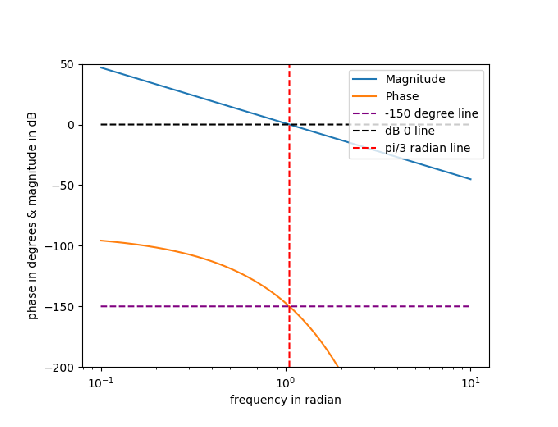
\includegraphics[width=\columnwidth]{./figs/ee18btech11038/ee18btech11038_graph.eps}
  \caption{}
  \label{fig:ee18btech11038_graph}
\end{figure}

\end{enumerate}
